\documentclass[conference]{IEEEtran}
\usepackage[T1]{fontenc}
\usepackage{amsmath}
\usepackage{graphicx}
\usepackage{booktabs}
\usepackage{cite}
\usepackage{url}
\usepackage[hidelinks]{hyperref}
\graphicspath{{figures/}}

\begin{document}

\title{Is Real Automotive Radar Sparse Enough for the Sparse FFT? A Study on RADIal}

\author{\IEEEauthorblockN{Daksh Shah}
\IEEEauthorblockA{Department of Electrical Engineering, National Institute of Technology Rourkela, India\\
daksh06shah2006@gmail.com \quad Code and data pipeline: \url{https://github.com/PLANETORIAN/Sparse-FFT-Radar}}}

\maketitle

\begin{abstract}
Sparse Fourier transforms promise to beat the FFT when a spectrum has few nonzero bins. I tested whether that holds for the Doppler FFT of a real high-definition automotive radar. Starting from the raw ADC files of the RADIal dataset, I built the range-Doppler chain and measured sparsity on three driving scenes. Between 63\% and 89\% of range rows have at most 8 Doppler peaks, but every row that contains a labelled vehicle has about 36 to 41, because Doppler-division multiplexing repeats each target 12 times. I then implemented the exactly-sparse FFT of Hassanieh et al.\ and ran it on real rows. At every computation cost it kept fewer Doppler peaks than a dense 256-point FFT or a simple energy-based row skip. At this transform size the dense FFT is the better hardware choice.
\end{abstract}



\section{Introduction}
A high-definition automotive radar produces a large data cube in every frame. In the RADIal dataset \cite{rebut2022radial} one frame has 512 range samples, 256 chirps and 16 receive channels. The Doppler stage runs one 256-point FFT for each range bin and channel, which is 8192 FFTs per frame and about 47\% of all FFT multiplications in the chain. A cheaper Doppler transform would matter on an FPGA.

\begin{figure}[b]
\centering
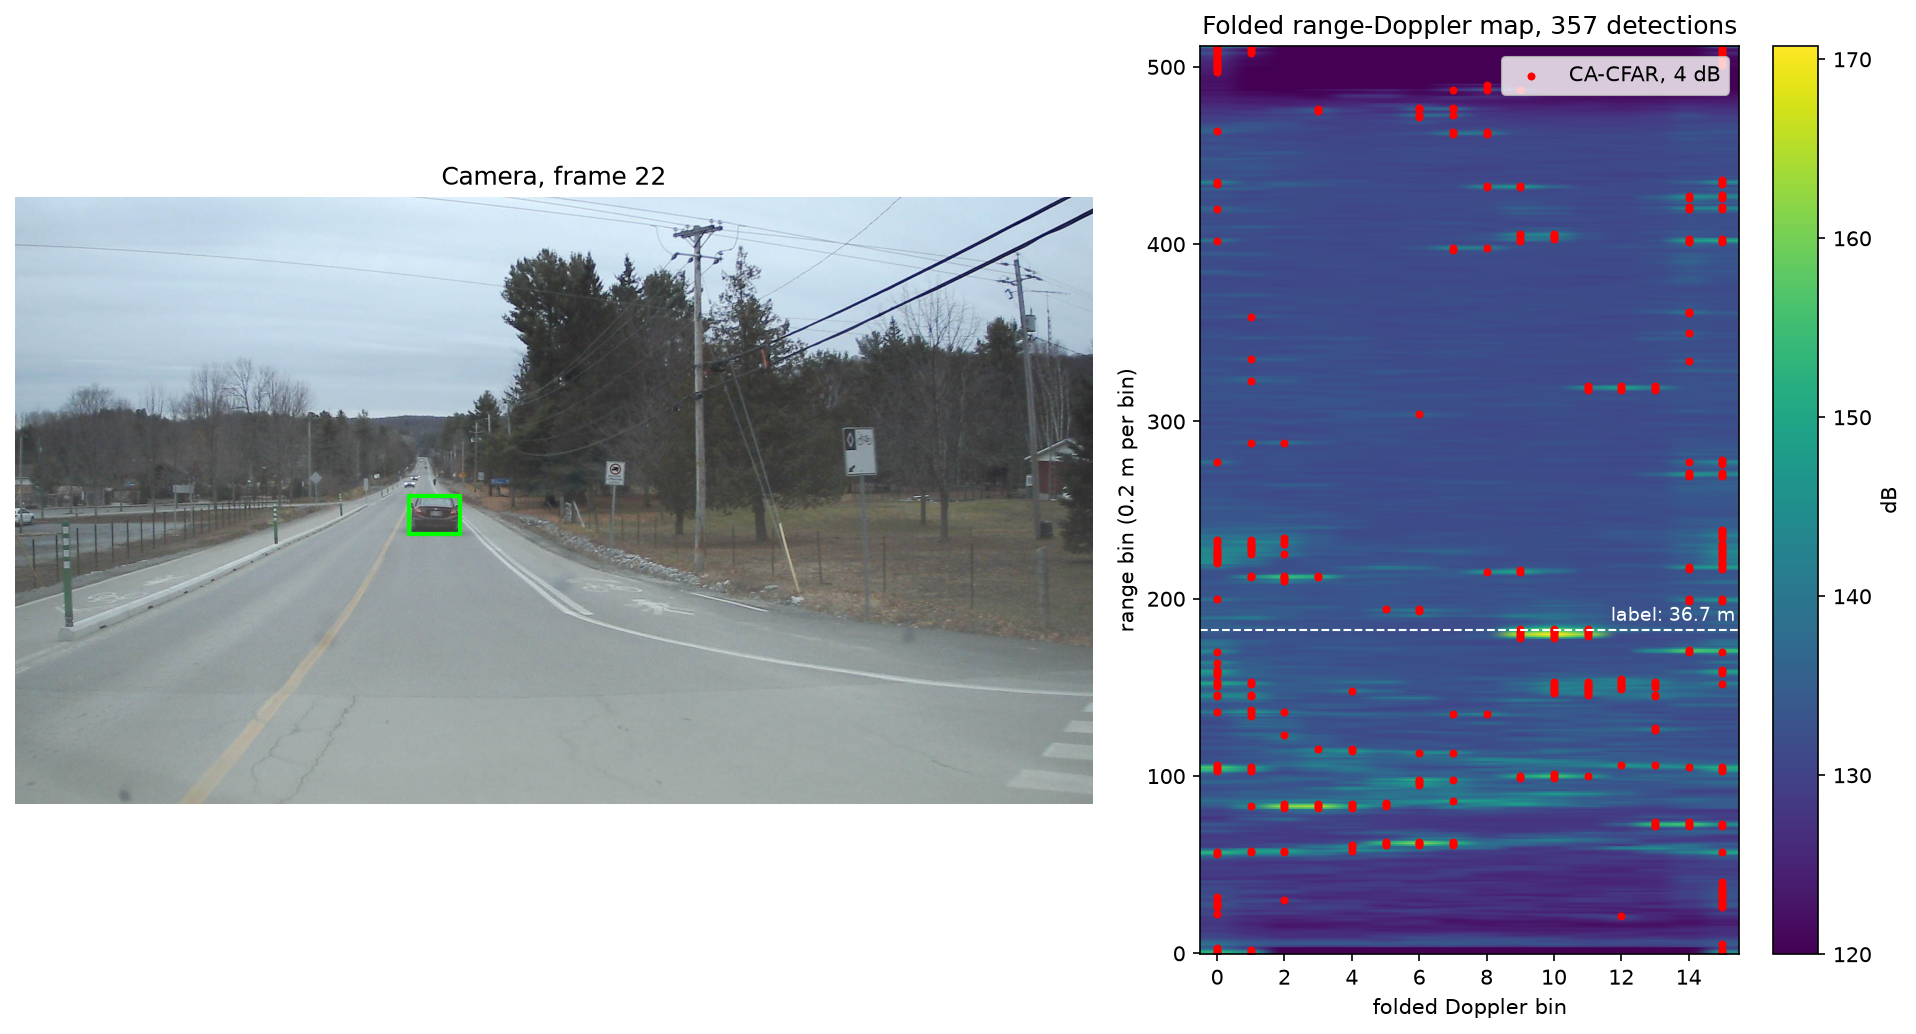
\includegraphics[width=\columnwidth]{fig_camera_rd_cfar.png}
\caption{Check of the chain on one countryside frame. Left: camera image with the dataset's label box. Right: range-Doppler map, Doppler folded over the DDM slots, with CA-CFAR detections (red) and the labelled range of 36.7\,m (dashed).}
\label{fig:camera}
\end{figure}

Sparse FFT algorithms \cite{hassanieh2012nearly,hassanieh2012simple} compute the $K$ largest Fourier coefficients of a length-$N$ signal in time that grows with $K$ instead of $N$. Their guarantees assume that $K$ is small. Whether a real radar row meets that assumption is an empirical question, and this report answers it for one radar. The scope is three sequences of one dataset and a transform size of $N = 256$.

\begin{figure}[t]
\centering
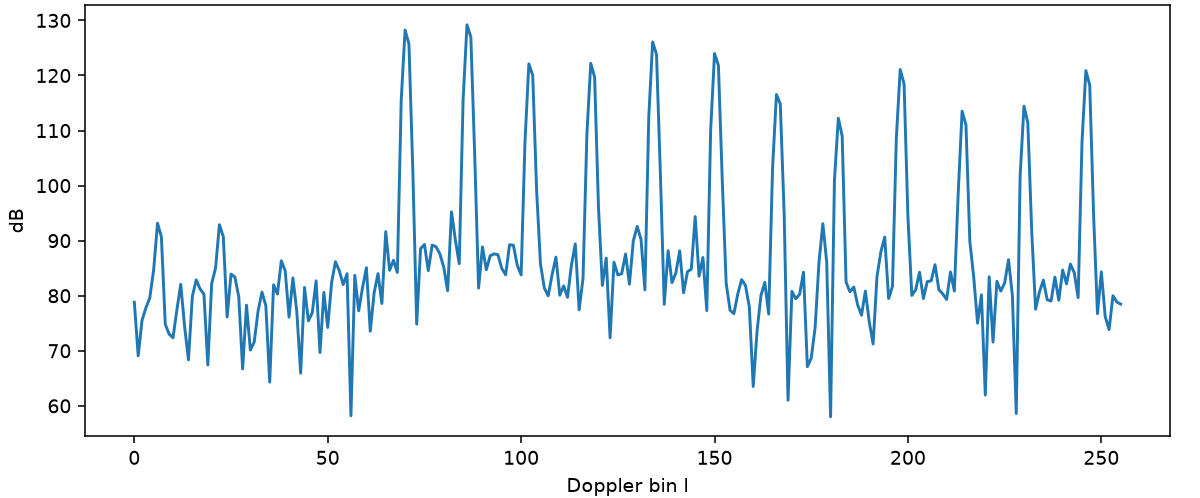
\includegraphics[width=\columnwidth]{fig_ddm_comb.png}
\caption{Doppler spectrum (dB against Doppler bin) of one range row that contains a vehicle, one receive channel. The single vehicle appears as 12 DDM copies, 16 bins apart.}
\label{fig:comb}
\end{figure}

I report three measurements:
\begin{enumerate}
\item how many Doppler peaks a range row holds in city, countryside and highway scenes, and how many it holds when a vehicle is present;
\item the computation and the success rate of an exactly-sparse FFT on synthetic rows with a known number of tones;
\item the share of real Doppler peaks the same algorithm keeps, against its computation, compared with a dense FFT and with skipping low-energy rows.
\end{enumerate}

\section{Data and Baseline Chain}
RADIal provides raw ADC samples from four radar chips, with camera images and vehicle labels \cite{rebut2022radial}. I used one city, one countryside and one highway sequence, with 576, 452 and 388 complete radar frames.

I wrote the chain from the raw files and did not use precomputed maps. Each frame is assembled from four chip blocks into a $512 \times 256 \times 16$ complex cube. After removing the mean of each channel, I apply a Hamming window and an FFT along range, then a Hamming window and an FFT along Doppler. One range bin is about 0.2\,m. I checked the chain by overlaying cell-averaging CFAR detections \cite{rohling1983cfar} and the dataset labels on the camera image for frames of all three scenes (Fig.~\ref{fig:camera}).

The radar separates its 12 transmitters by Doppler-division multiplexing (DDM). Each target therefore appears 12 times along Doppler, 16 bins apart (Fig.~\ref{fig:comb}). This property decides most of what follows.


\section{How Sparse Is Real Radar?}
\subsection{A measure that misleads}
My first measure was $K_{90}$, the smallest number of bins that hold 90\% of the energy of the $512 \times 256$ power map. It ranked the scenes backwards: 5.3\% of bins for the city, 13.3\% for the countryside and 46.1\% for the highway, against 84.6\% for pure noise passed through the same chain. The highway is the emptiest scene, so its peaks hold the smallest share of the total energy, and $K_{90}$ has to reach into the flat noise floor. $K_{90}$ measures how energy splits between peaks and floor. It does not count peaks.

\subsection{Peaks per range row}
A Doppler sparse FFT would replace one 256-point FFT per range row. The quantity that matters is therefore $K$, the number of bins in a row that lie more than 10\,dB above that row's median power, summed over the 16 channels. Pure noise gives $K = 0$ in every row.

\begin{figure}[t]
\centering
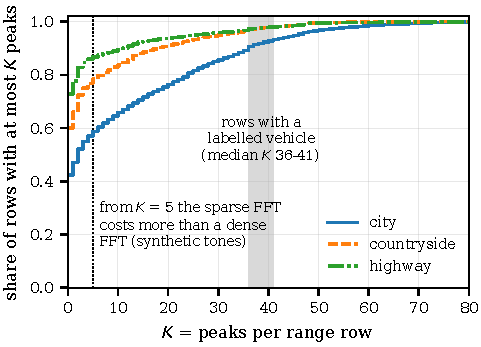
\includegraphics[width=\columnwidth]{fig_row_k_cdf.pdf}
\caption{Share of range rows with at most $K$ Doppler peaks ($K$ = bins more than 10\,dB above the row median, 256 bins per row), every 5th frame of each sequence. Most rows are nearly empty, but rows with a vehicle lie far to the right.}
\label{fig:cdf}
\end{figure}

\begin{table}[t]
\caption{Doppler peaks per range row, $K$, at 10\,dB}
\label{tab:k}
\centering
\begin{tabular}{lccc}
\toprule
 & City & Countryside & Highway \\
\midrule
Frames / rows & 116 / 59\,392 & 91 / 46\,592 & 78 / 39\,936 \\
Median $K$ & 2 & 0 & 0 \\
90th percentile of $K$ & 36 & 18 & 11 \\
Rows with $K = 0$ & 42\% & 60\% & 73\% \\
Rows with $K \le 8$ & 63.2\% & 81.9\% & 88.5\% \\
\midrule
Labelled vehicles used & (too few) & 55 & 32 \\
Median $K$, vehicle rows & -- & 41 & 36 \\
Vehicle rows with $K \le 8$ & -- & 0\% & 0\% \\
\bottomrule
\end{tabular}
\end{table}

Fig.~\ref{fig:cdf} and Table~\ref{tab:k} show that most rows are sparse, and that the highway is the sparsest scene and the city the least sparse. The ranking is the same at a 6\,dB threshold, although the share of rows with $K \le 8$ drops to 39.9\%, 56.6\% and 71.4\%.

\begin{figure*}[t]
\centering
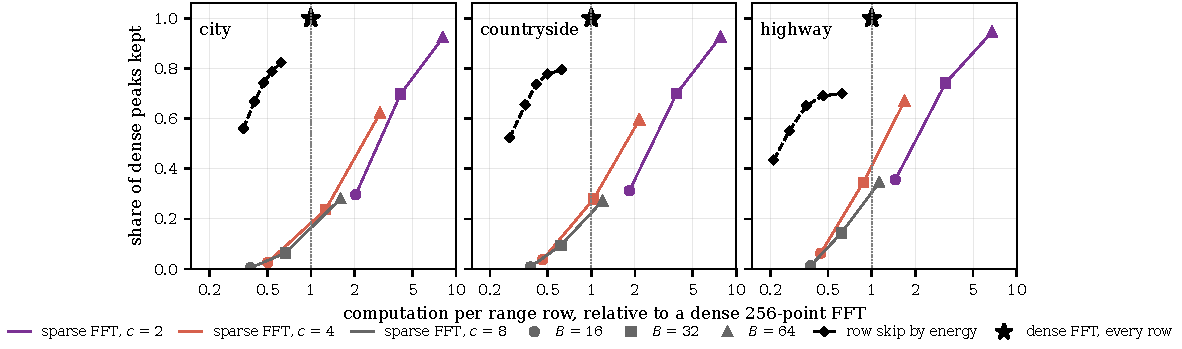
\includegraphics[width=\textwidth]{fig_recall_vs_cost.pdf}
\caption{Share of dense Doppler peaks (more than 10\,dB above the row median) kept, against computation per range row relative to a 256-point FFT. Sparse FFT with $B$ buckets and occupancy threshold $c$; dashed: dense FFT only on rows whose energy exceeds $a$ times the median row energy, $a = 3$ to 1. In every scene the sparse FFT lies below and to the right of both alternatives.}
\label{fig:recall}
\end{figure*}

\subsection{Rows that contain a vehicle}
The sparse rows are the empty ones. For labelled vehicles whose radar frame I could identify with confidence, the row at the vehicle's range has a median $K$ of 41 in the countryside and 36 on the highway. No vehicle row had $K \le 8$. The number follows from DDM: 12 copies, each about 3 bins wide after the Hamming window. A sparse FFT must therefore be compared with the trivial alternative of skipping empty rows, not only with the dense FFT.

\section{Sparse FFT on a Doppler Row}
\subsection{Algorithm}
I implemented the exactly-sparse algorithm of Hassanieh, Indyk, Katabi and Price \cite{hassanieh2012nearly}. One round works as follows. The samples are read in steps of a random odd $\sigma$, which moves bin $f$ to $\sigma f \bmod N$. They are multiplied by a window whose spectrum is flat over $N/B$ neighbouring bins, folded to $B$ values and passed through one $B$-point FFT. This gives $B$ buckets, each the sum of a band of permuted bins. The same is done with the samples shifted by one. If a bucket holds a single tone, the phase between its two values gives the tone's bin,
\begin{equation}
\hat{p} = \mathrm{round}\!\left(\frac{N}{2\pi}\,\arg\frac{u_1[j]}{u_0[j]}\right), \qquad \hat{f} = \sigma^{-1}\hat{p} \bmod N ,
\end{equation}
where $u_0[j]$ and $u_1[j]$ are the values of bucket $j$ without and with the shift. Found tones are subtracted, and the round repeats with a new $\sigma$.

Simple buckets made by keeping every 16th sample cannot work on this radar. They add the bins that are 16 apart, so all 12 DDM copies of a target fall into one bucket. The band-shaped buckets of the flat window separate them.

For real rows I process the 16 channels together. Bucket power is summed over channels, the phase is averaged over channels, and a bucket counts as occupied if its power exceeds $c$ times the median bucket power.

\subsection{Synthetic rows}
I count complex multiplications. A dense radix-2 FFT of length 256 costs 1024. One round of the sparse FFT costs 378, 546 and 862 for $B = 16$, 32 and 64, because the flat window alone reads 141 or more of the 256 samples in each of the two hashings. Table~\ref{tab:syn} gives the result for noise-free tones on exact bins. The sparse FFT is cheaper than the dense FFT for one tone and more expensive from five tones. A row with 36 tones needs $B = 64$, costs about ten times the dense FFT and still fails in 9\% of trials.

\begin{table}[t]
\caption{Synthetic rows: share recovered exactly / median multiplications (dense FFT: 1024)}
\label{tab:syn}
\centering
\begin{tabular}{lcccc}
\toprule
$B$ & $K = 1$ & $K = 5$ & $K = 12$ & $K = 36$ \\
\midrule
16 & 1.00 / 378 & 1.00 / 1512 & 0.93 / 4536 & 0.00 / 4536 \\
32 & 1.00 / 546 & 1.00 / 1638 & 1.00 / 6552 & 0.00 / 6552 \\
64 & 1.00 / 862 & 1.00 / 2586 & 1.00 / 10\,344 & 0.91 / 10\,344 \\
\bottomrule
\end{tabular}
\end{table}

\subsection{Real rows}

On real data I took every 25th frame of each sequence. A dense peak is a local maximum more than 10\,dB above the row median. It counts as kept if the sparse output exceeds the same threshold within one bin. With $c = 4$ and all 512 rows, the sparse FFT kept 3\%, 24\% and 61\% of the city peaks for $B = 16$, 32 and 64, at 0.51, 1.29 and 2.99 times the dense cost. The highway was its best case: 70\% of peaks at 1.70 times the dense cost.

Fig.~\ref{fig:recall} adds two checks. Changing $c$ moves the sparse FFT along one trade-off: $c = 2$ keeps 92\% to 95\% of the peaks with $B = 64$, at 6.7 to 8.1 times the dense cost. The dashed curve is a row skip that needs no FFT to decide: the dense FFT runs only on rows whose energy exceeds a multiple $a$ of the median row energy. I first assumed that skipping empty rows would keep every peak. It does not. With $a = 1$ it keeps 82\%, 79\% and 70\% of the peaks at 0.62 of the dense cost, because weak peaks sit in low-energy rows. At a similar cost the sparse FFT keeps 6\% to 14\%.

Two effects explain the low recall. Vehicle rows hold about 36 peaks, more than a small $B$ can separate. And each bucket sums $L = N/B$ bins, so it also sums $L$ bins of noise. A peak is then compared with $10\log_{10} L$ more noise: 12\,dB for $B = 16$ and 6\,dB for $B = 64$. A peak 10\,dB above the floor of its row disappears in a 16-bin bucket.

\section{Computation Cost}
The cost model counts the window multiplications and the $B$-point FFT of each hashing, two hashings per round and two multiplications per bucket for the phase test. It counts the subtraction of found tones as free, which favours the sparse FFT. Even so, the sparse FFT is cheaper than the dense FFT only for rows with one or very few tones, and those rows are the ones a row skip removes for 0.125 of a dense FFT. I did not synthesise either design. The comparison is an operation count, and area, memory and latency on an FPGA remain to be measured.

\section{Limitations and Next Steps}
The study covers three sequences of one dataset and one radar. $K$ depends on the threshold: between 10\,dB and 6\,dB the share of rows with $K \le 8$ changes by about 20 points, although the ranking of the scenes does not. The vehicle-row result rests on 55 and 32 labelled vehicles; in the city sequence, dropped radar blocks left too few labels that I could match to a frame. Static clutter was not removed, so $K$ includes it. The algorithm I tested assumes an exactly sparse spectrum, and the noise-tolerant variants \cite{hassanieh2012nearly,hassanieh2012simple} may behave differently, at a higher cost. Finally, $N = 256$ is small for a sparse FFT: the window alone reads more than half the samples.

Three next steps follow. A sparse transform that treats the 12 DDM copies as one target, since their spacing is known, would reduce the 12 peaks of each target to one. A two-dimensional transform over range and Doppler would work at a larger $N$, where sparse methods have more room. And an HLS implementation would replace the operation count with measured FPGA cost.

\begin{thebibliography}{1}
\bibitem{rebut2022radial}
J.~Rebut, A.~Ouaknine, W.~Malik, and P.~P\'erez, ``Raw high-definition radar for multi-task learning,'' in \emph{Proc. IEEE/CVF Conf. Computer Vision and Pattern Recognition (CVPR)}, 2022, pp. 17021--17030.

\bibitem{hassanieh2012nearly}
H.~Hassanieh, P.~Indyk, D.~Katabi, and E.~Price, ``Nearly optimal sparse Fourier transform,'' in \emph{Proc. 44th ACM Symp. Theory of Computing (STOC)}, 2012, pp. 563--578, doi: 10.1145/2213977.2214029.

\bibitem{hassanieh2012simple}
H.~Hassanieh, P.~Indyk, D.~Katabi, and E.~Price, ``Simple and practical algorithm for sparse Fourier transform,'' in \emph{Proc. 23rd ACM-SIAM Symp. Discrete Algorithms (SODA)}, 2012, pp. 1183--1194.

\bibitem{rohling1983cfar}
H.~Rohling, ``Radar CFAR thresholding in clutter and multiple target situations,'' \emph{IEEE Trans. Aerosp. Electron. Syst.}, vol. AES-19, no. 4, pp. 608--621, Jul. 1983.
\end{thebibliography}

\end{document}
